%\documentclass[italian]{scrreprt}
\documentclass[italian,a4paper,12pt]{scrreprt}
\usepackage[T1]{fontenc}
\usepackage[utf8]{inputenc}
\usepackage{geometry}
\usepackage{graphicx}
\usepackage{forest}
\setcounter{secnumdepth}{3}
\setcounter{tocdepth}{1}
\usepackage{float}
\usepackage{babel}
\usepackage{microtype} % migliora espansione dei font. Suggerito su ``L'arte di scrivere in LaTeX, pag. 45''
\usepackage{indentfirst} % indentazione anche su primo paragrafo.  Suggerito su ``L'arte di scrivere in LaTeX, pag. 45''
\usepackage{booktabs} % serve per le tabelle.   Suggerito su ``L'arte di scrivere in LaTeX, pag. 85''
\usepackage{caption} % serve per le tabelle.   Suggerito su ``L'arte di scrivere in LaTeX, pag. 85''



\geometry{textheight=24.2cm,textwidth=16cm}
\pagestyle{headings}
\frenchspacing

\date{}

\title{
\huge Guida all'uso della piattaforma di prenotazione sale
\\ Booked
}
\subtitle{Versione super amministratori}
\author{Rilascio 0.07 \\
Germano Massullo}

\makeindex

\begin{document}
\maketitle
\tableofcontents
\chapter{Introduzione}
La presente guida ha come oggetto l'utilizzo della piattaforma Booked scheduler
per gestione elettronica delle prenotazioni di aule dell'ateneo.
Per un'agevole comprensione del testo, vengono introdotti di seguito alcuni concetti preliminari.
Booked gestisce tre tipi fondamentali di oggetti:
\begin{itemize}
 \item calendari;
 \item risorse;
 \item prenotazioni.
\end{itemize}
\paragraph*{Calendari}\mbox{}\\ %per andare a capo dopo nome paragrafo.
I calendari presenti sono:
\begin{itemize}
 \item Default;
 \item Economia;
 \item Ingegneria;
 \item Lettere;
 \item Medicina;
 \item Scienze.
\end{itemize}

in maniera tale da separare le esigenze di prenotazione delle varie macro aree d'ateneo.
Il calendario ``Default'' è un calendario predefinito e vuoto, che appare quando si accede
alla pagina web dei calendari, pertanto occorre scegliere quello di propria competenza.

\paragraph*{Risorse}\mbox{}\\ %per andare a capo dopo nome paragrafo.
Booked gestisce prenotazioni di risorse: esse possono essere laboratori, laboratori,
mezzi di trasporto, aule didattiche, ecc. Queste ultime pertanto, verranno viste dal
programma come delle risorse.


\paragraph*{Prenotazioni}\mbox{}\\ %per andare a capo dopo nome paragrafo.
Le prenotazioni vengono effettuate operando sulla pagina che mostra il calendario: si sceglie
la risorsa da prenotare e si impostano le proprie preferenze.
\chapter{Prenotazioni}
Per effettuare una prenotazione, cliccare la voce ``Calendario'' nel menù in alto alla pagina web.
Selezionare il calendario di propria competenza
\begin{figure}[H]
\centering{}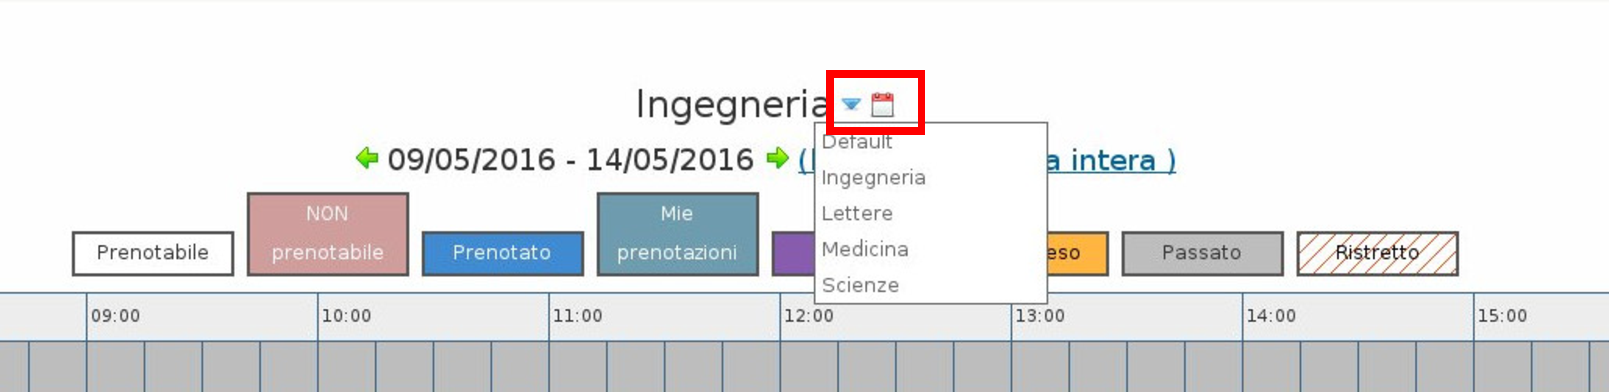
\includegraphics[scale=0.5]{Immagini/calendari_selezione.pdf}
\normalsize
\caption{}
\label{fig:calendari_selezione.pdf}
\end{figure}

e scorrere la pagina fino a trovare la data adatta alla prenotazione. Sulle righe
sono presenti tutte le risorse (aule) disponibili.
Per iniziare a creare una prenotazione cliccare su un quadratino qualsiasi nella fascia oraria
dell'aula desiderata. È possibile modificare i dettagli orari nella schermata
successiva.

Per fissare una prenotazione su più giorni della settimana, andare nella zona ``Ripeti'' come in Figura
\ref{fig:prenotazione_ripetizione_1.pdf}

\begin{figure}[H]
\centering{}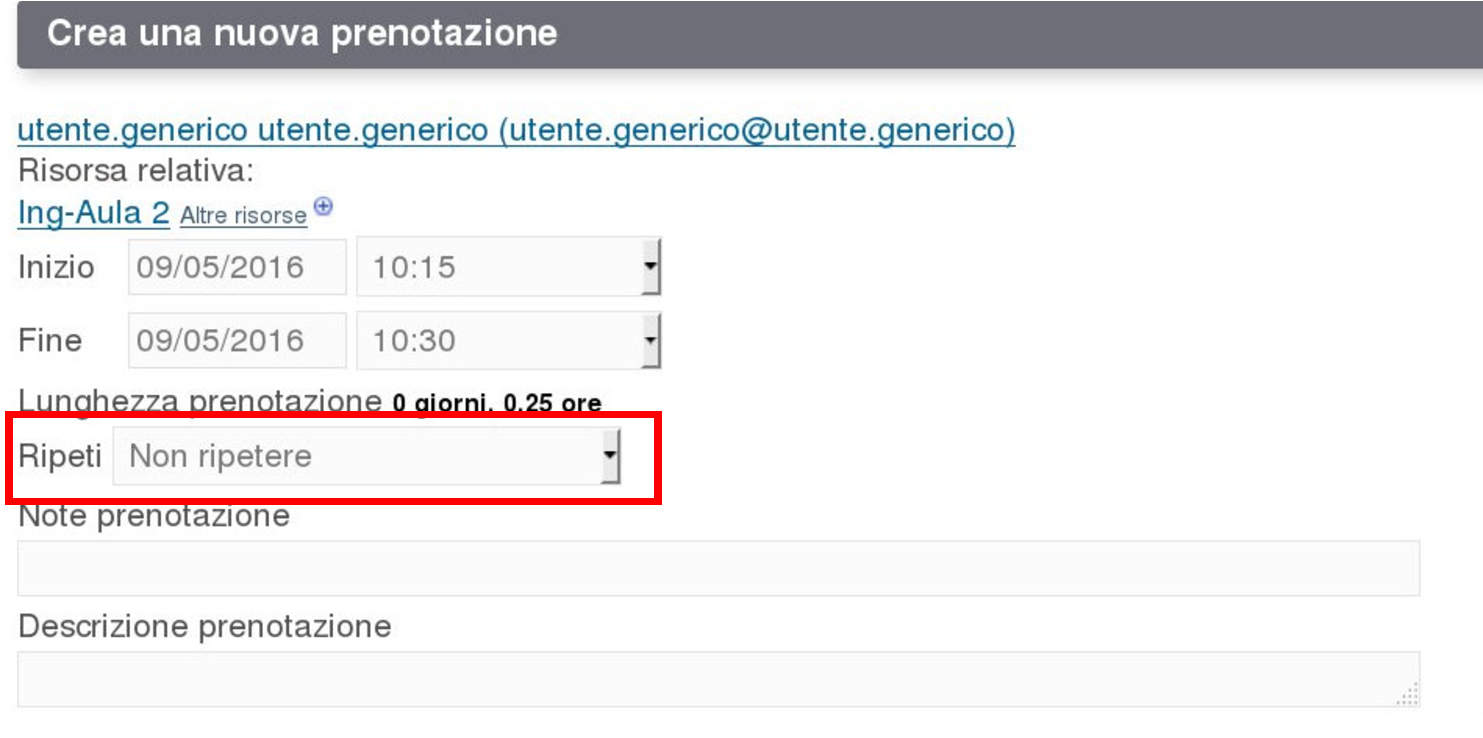
\includegraphics[scale=0.5]{Immagini/prenotazione_ripetizione_1.pdf}
\normalsize
\caption{}
\label{fig:prenotazione_ripetizione_1.pdf}
\end{figure}

e cliccare su ``Settimanale''

\begin{figure}[H]
\centering{}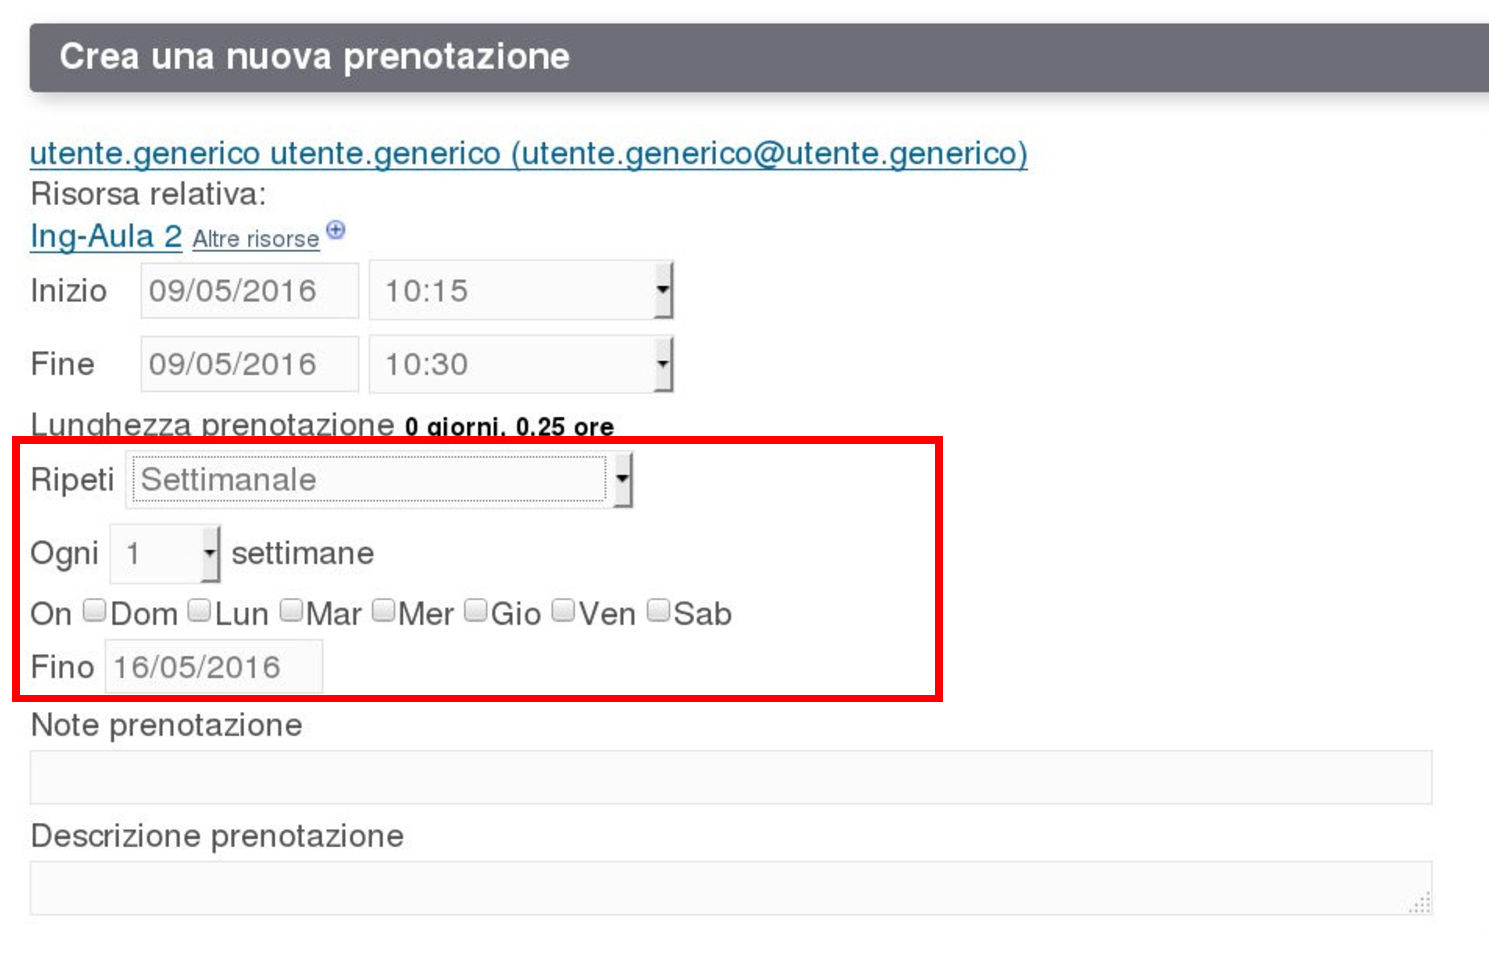
\includegraphics[scale=0.5]{Immagini/prenotazione_ripetizione_2.pdf}
\normalsize
\caption{}
\label{fig:prenotazione_ripetizione_2.pdf}
\end{figure}


La scritta ``Note prenotazione'' significa ``Nome prenotazione''. Vi è un errore di traduzione
del software, che verrà corretto a breve.
Non dimenticare di aggiungere il corso di studi della materia e l'anno corrispondente.


\begin{figure}[H]
\centering{}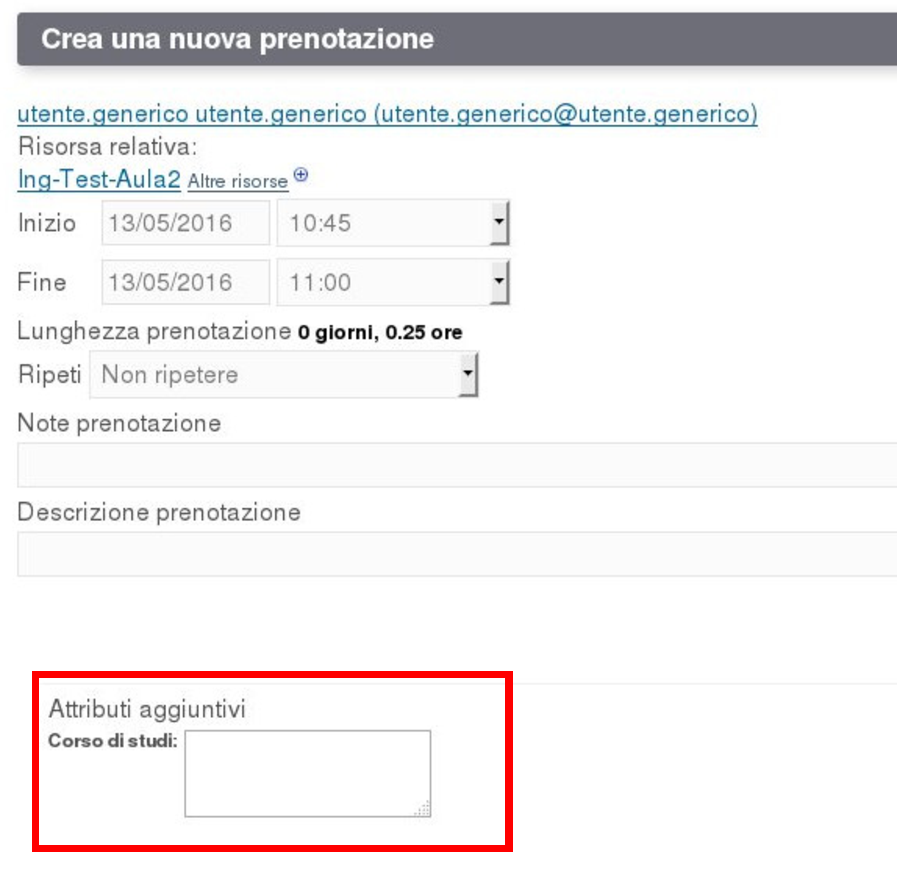
\includegraphics[scale=0.5]{Immagini/prenotazione_attributi.pdf}
\normalsize
\caption{}
\label{fig:prenotazione_attributi.pdf}
\end{figure}

Un esempio può essere

\begin{figure}[H]
 \centering{} Ingegneria informatica II anno
\normalsize
\end{figure}

Nel caso la prenotazione riguardi più corsi di studi, metterne uno per riga
\input{Capitoli/Amministrazione/Gestione/Gestione}
\section{Calendari}
La gestione dei calendari è accessibile mediante apposito menù come in figura
\ref{fig:amministratore_menu_generale_selezione_calendari.pdf}
\begin{figure}[H]
\centering{}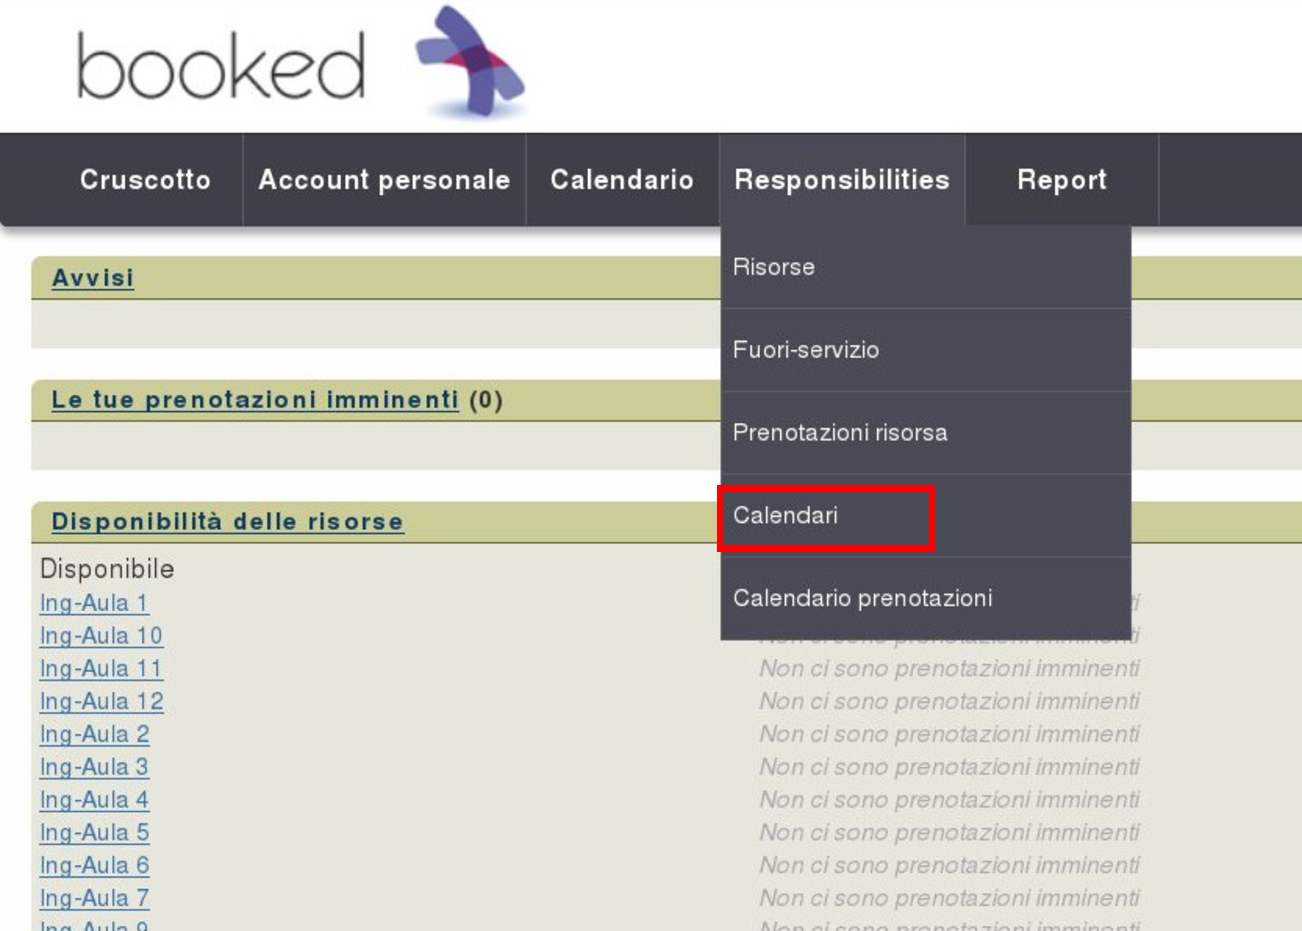
\includegraphics[scale=0.5]{Immagini/amministratore_menu_generale_selezione_calendari.pdf}
\normalsize
\caption{}
\label{fig:amministratore_menu_generale_selezione_calendari.pdf}
\end{figure}

all'interno è possibile gestire le fasce orarie disponibili, ed il frazionamento degli intervalli orari.
Non confondere la gestione calendari con la gestione delle prenotazioni, che si fa altrove.
Dopo la creazione di un nuovo calendario, accedere all'opzione ``cambia layout'' e controllare che il fuso
orario sia Europe/Rome.
\section{Risorse}
Le risorse sono accessibili mediante apposito menù
\begin{figure}[H]
\centering{}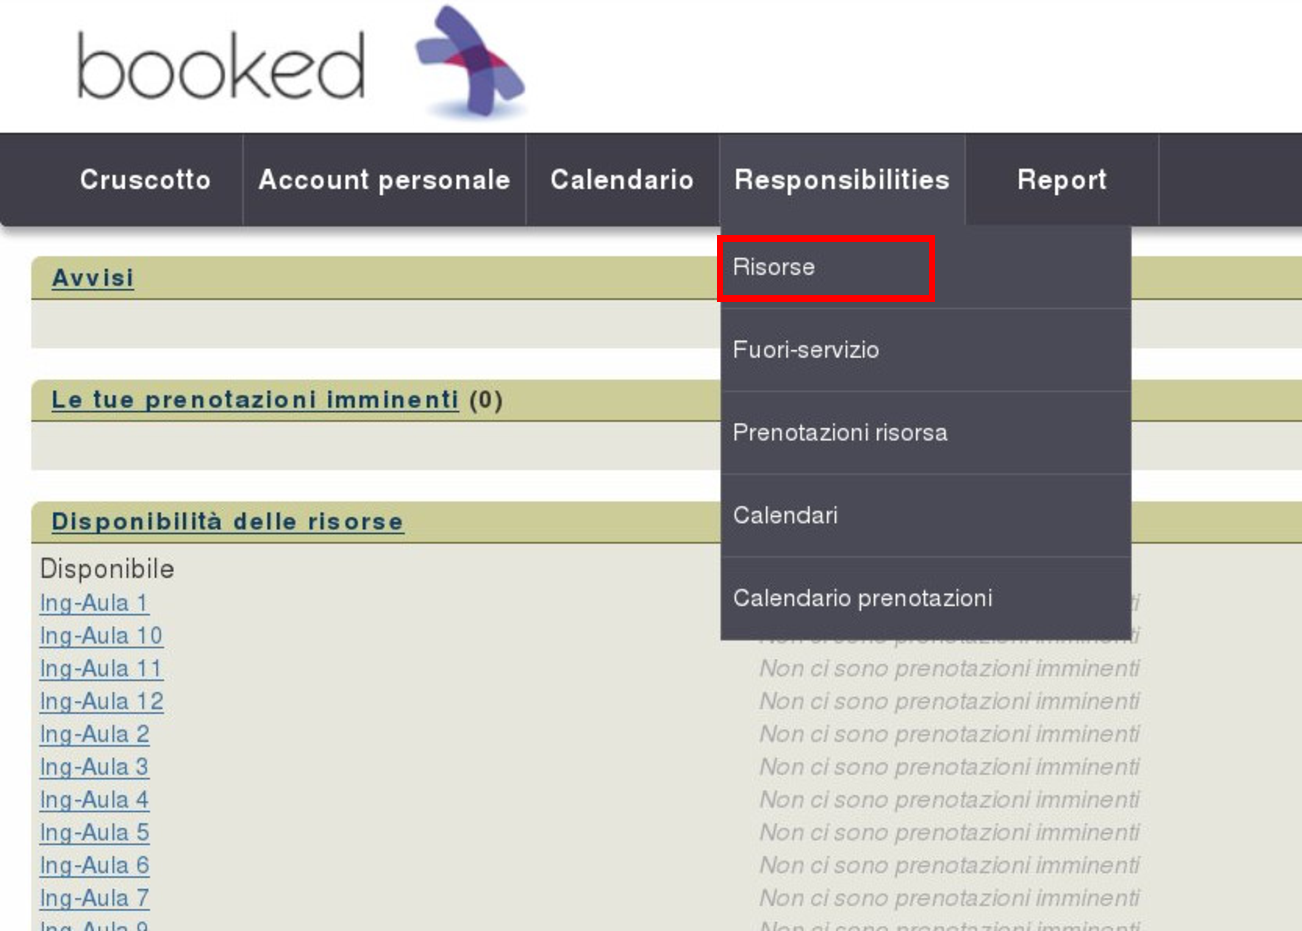
\includegraphics[scale=0.5]{Immagini/amministratore_menu_generale_selezione_risorse.pdf}
\normalsize
\caption{}
\label{fig:amministratore_menu_generale_selezione_risorse.pdf}
\end{figure}

\subsection{Creazione nuove risorse}
Per aggiungere nuove risorse, scorrere il menù risorse fino ad ottenere la visuale di
Figura \ref{fig:risorse_vista_generale_creazione.pdf}
\begin{figure}[H]
\centering{}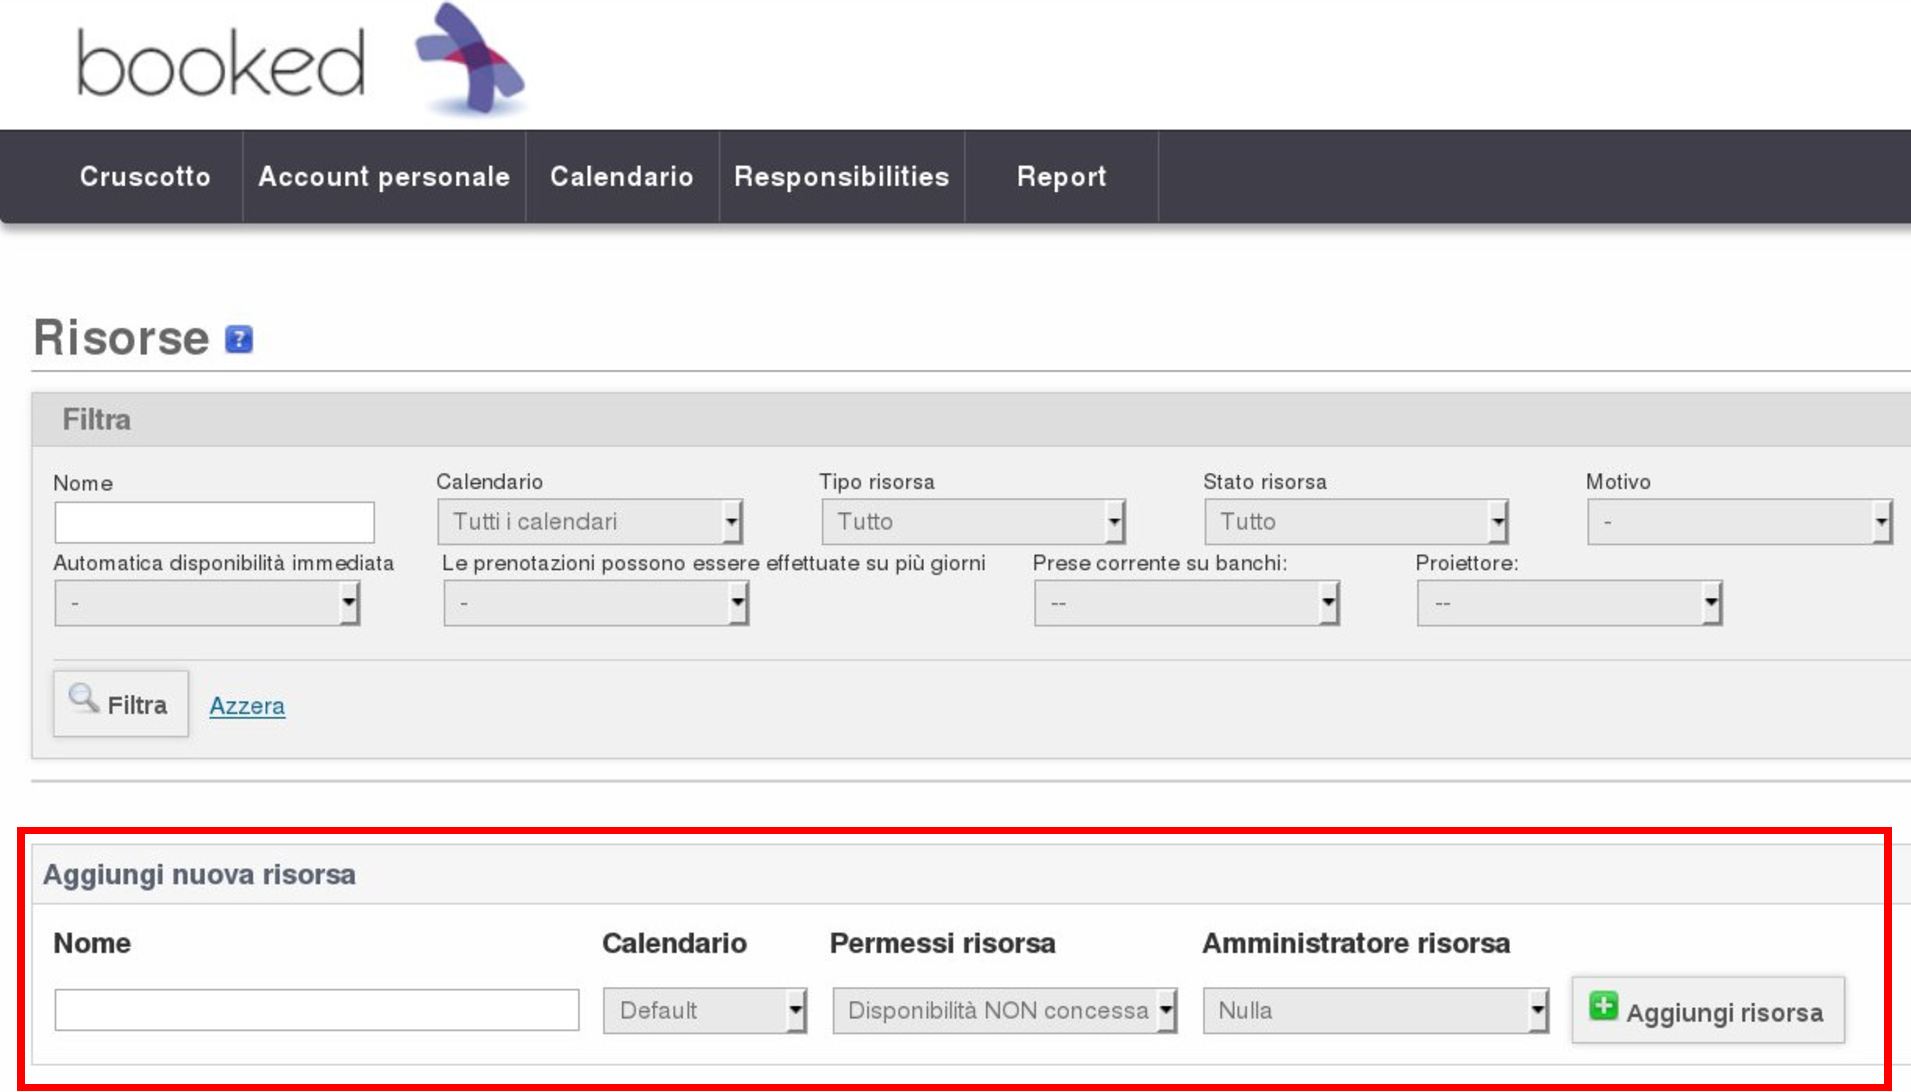
\includegraphics[scale=0.5]{Immagini/risorse_vista_generale_creazione.pdf}
\normalsize
\caption{}
\label{fig:risorse_vista_generale_creazione.pdf}
\end{figure}

\paragraph*{Nome}\mbox{}\\ %per andare a capo dopo nome paragrafo.
Per mantenere una coerenza tra tutte le varie macro aree d'ateneo, si deve rispettare una precisa
nomenclatura nella creazione di nuove risorse, come nel seguente esempio:
\begin{figure}[H]
\centering{}Ing-Aula A1
\normalsize
\end{figure}
perciò:
\begin{enumerate}
 \item prime tre lettere del nome della macro area, con la prima in formato maiuscolo;
 \item trattino, facendo attenzione a non immettere spazi ai lati;
 \item nome della risorsa.
\end{enumerate}

\paragraph*{Calendario}\mbox{}\\ %per andare a capo dopo nome paragrafo.
Ogni risorsa di Booked deve essere assegnata ad uno ed un solo calendario.
Selezionare quello di propria competenza.

\paragraph*{Permessi risorsa}\mbox{}\\ %per andare a capo dopo nome paragrafo.
\begin{itemize}
 \item Disponibilità NON concessa automaticamente: significa che gli utenti che non hanno privilegi
 di amministratore, non potranno fare richieste prenotazioni della risorsa;
 \item Disponibilità concessa automaticamente: gli utenti sono liberi di richiedere prenotazioni.
\end{itemize}
Per quanto riguarda l'approvazione delle prenotazioni leggere il paragrafo
``Gestione risorse esistenti''

\paragraph*{Amministratore risorsa}\mbox{}\\ %per andare a capo dopo nome paragrafo.
Serve a selezionare il gruppo di amministratori che dovrà gestire la risorsa. La mancata selezione
di tale opzione non renderà visibile la risorsa nel proprio elenco.
Scegliere il gruppo
\begin{figure}[H]
\centering{}Amministratori Calendario e Risorse
\normalsize
\end{figure}
che appartiene alla propria macro area


\newpage
\subsection{Gestione risorse esistenti}
La gestione di una risorsa è possibile cliccando sul menù nella seguente figura.


\begin{figure}[H]
\centering{}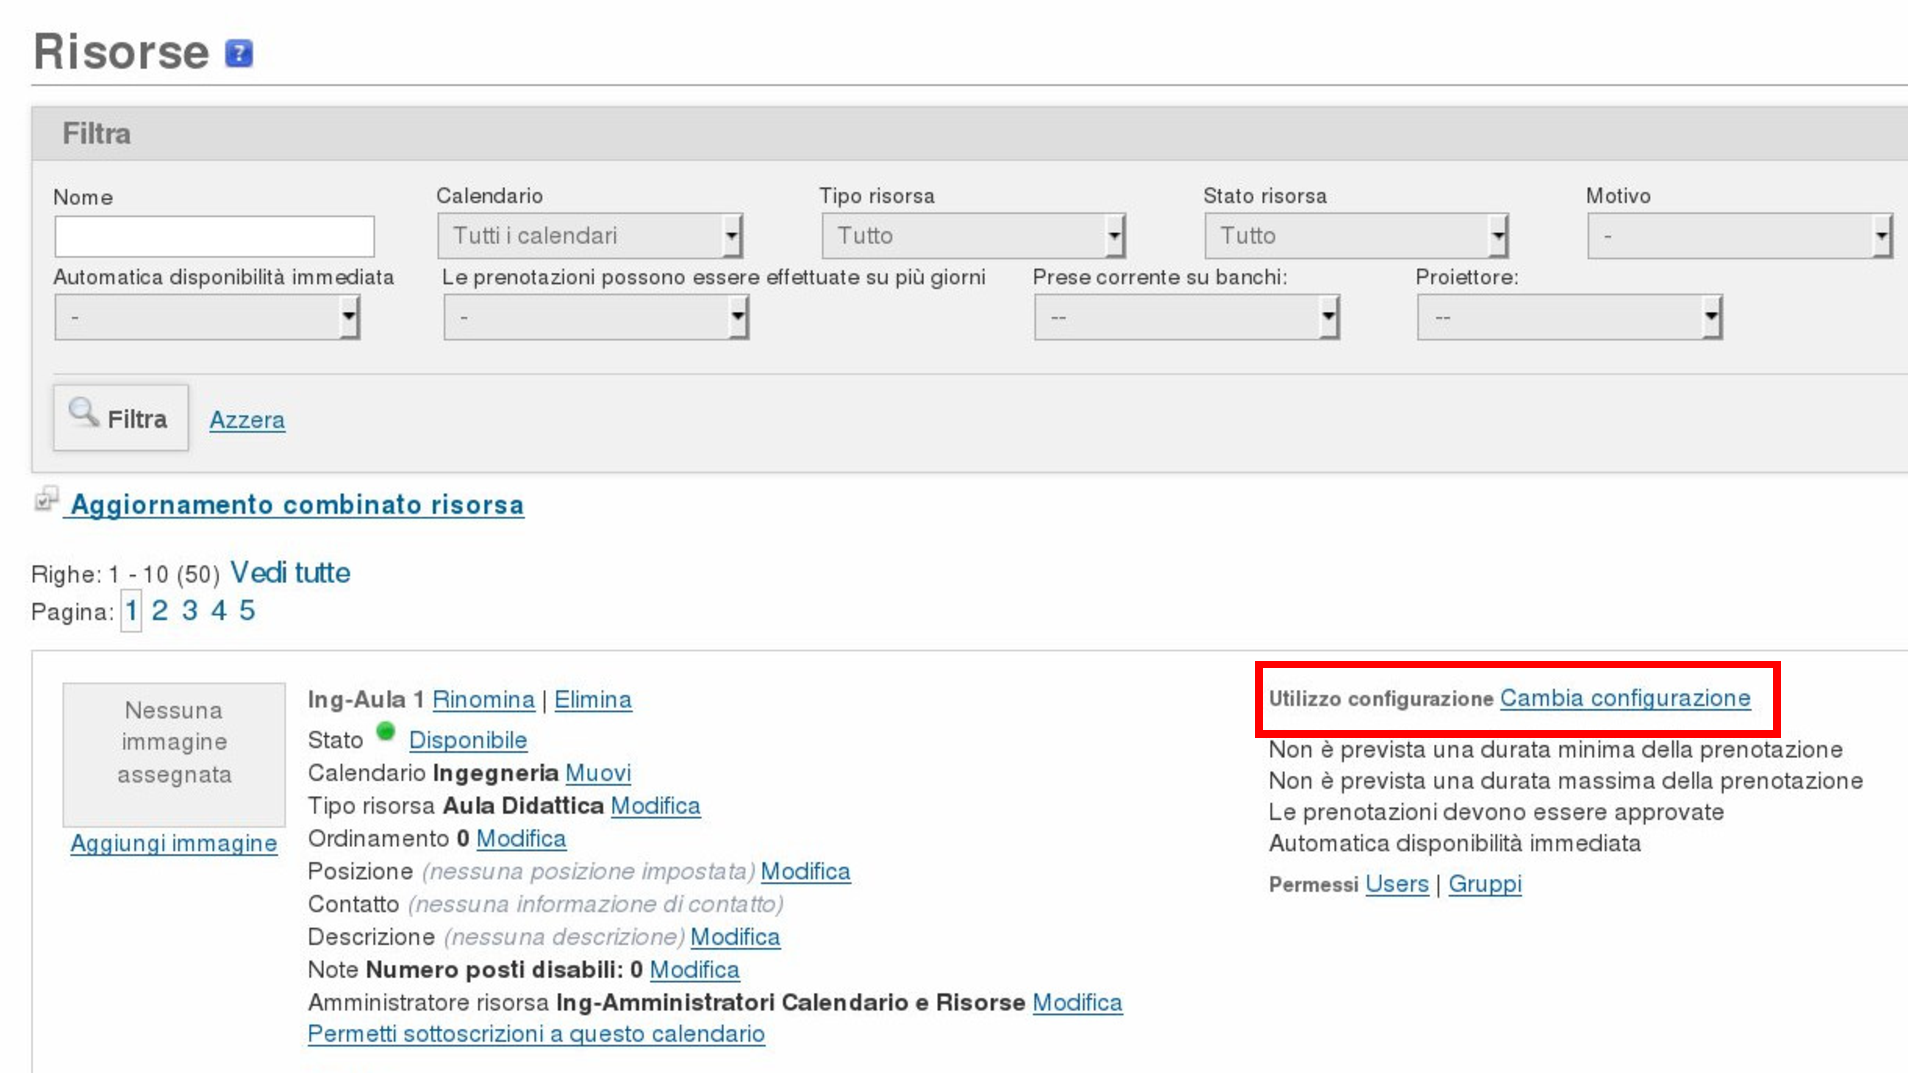
\includegraphics[scale=0.5]{Immagini/risorsa_selezione_configurazione.pdf}
\normalsize
\caption{}
\label{fig:risorsa_selezione_configurazione.pdf}
\end{figure}

Dato che Booked può gestire più tipi di risorse (ad esempio, mezzi di trasporto, aule),
dopo la creazione di nuove risorse, occorre assegnare loro una tipologia. Nel caso delle
aule selezionare ``Aula Didattica''.
Inoltre per assicurarsi che esse siano disponibili per chi effettua le prenotazioni,
si deve selezionare la proprietà ``Automatica disponibilità immediata (Sì)'', come in figura
\ref{fig:risorsa_configurazione_proprieta_disponibilita.pdf}

\begin{figure}[H]
\centering{}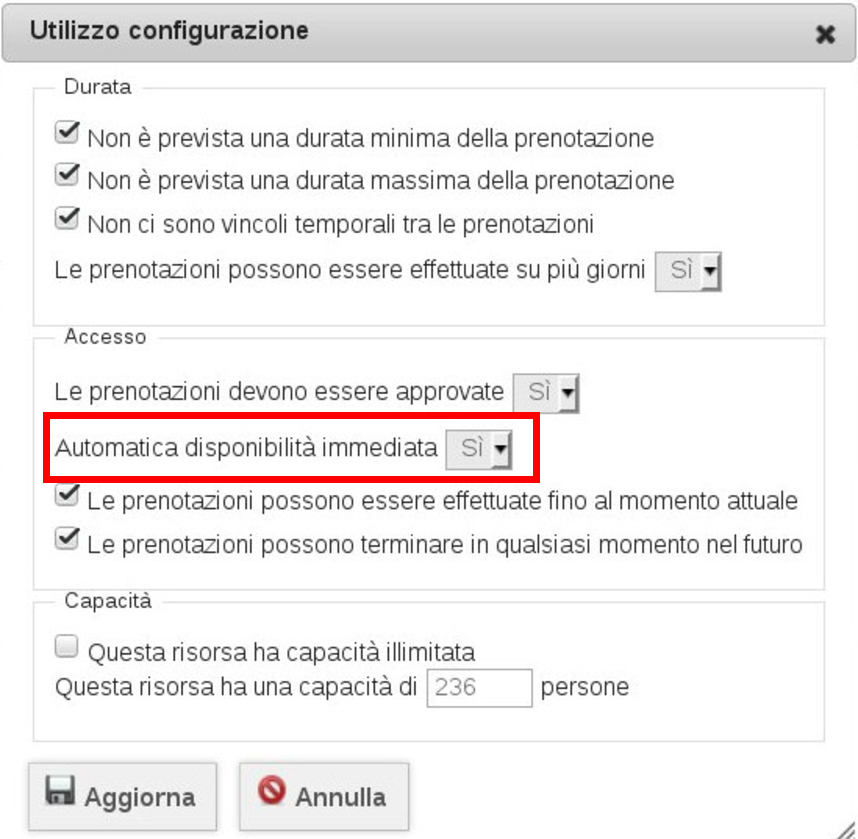
\includegraphics[scale=0.7]{Immagini/risorsa_configurazione_proprieta_disponibilita.pdf}
\normalsize
\caption{}
\label{fig:risorsa_configurazione_proprieta_disponibilita.pdf}
\end{figure}

Affinché la prenotazione di un utente debba passare dal vaglio dell'amministratore,
occorre selezionare la proprietà
Le prenotazioni devono essere approvate (Sì), come in figura
\ref{fig:risorsa_configurazione_proprieta_approvazione.pdf}

\begin{figure}[H]
\centering{}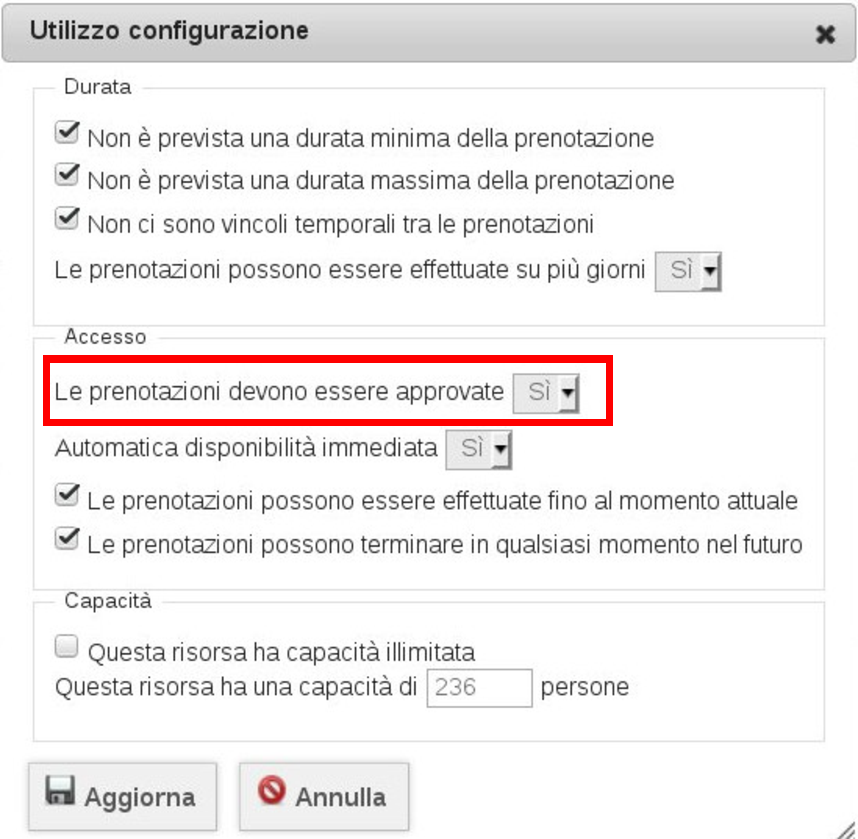
\includegraphics[scale=0.7]{Immagini/risorsa_configurazione_proprieta_approvazione.pdf}
\normalsize
\caption{}
\label{fig:risorsa_configurazione_proprieta_approvazione.pdf}
\end{figure}

Nel caso si voglia impostare proprietà di più risorse contemporaneamente, si può cliccare su
``Aggiornamento combinato risorsa'' come in figura
\ref{fig:risorsa_selezione_configurazione_multipla.pdf}

\begin{figure}[H]
\centering{}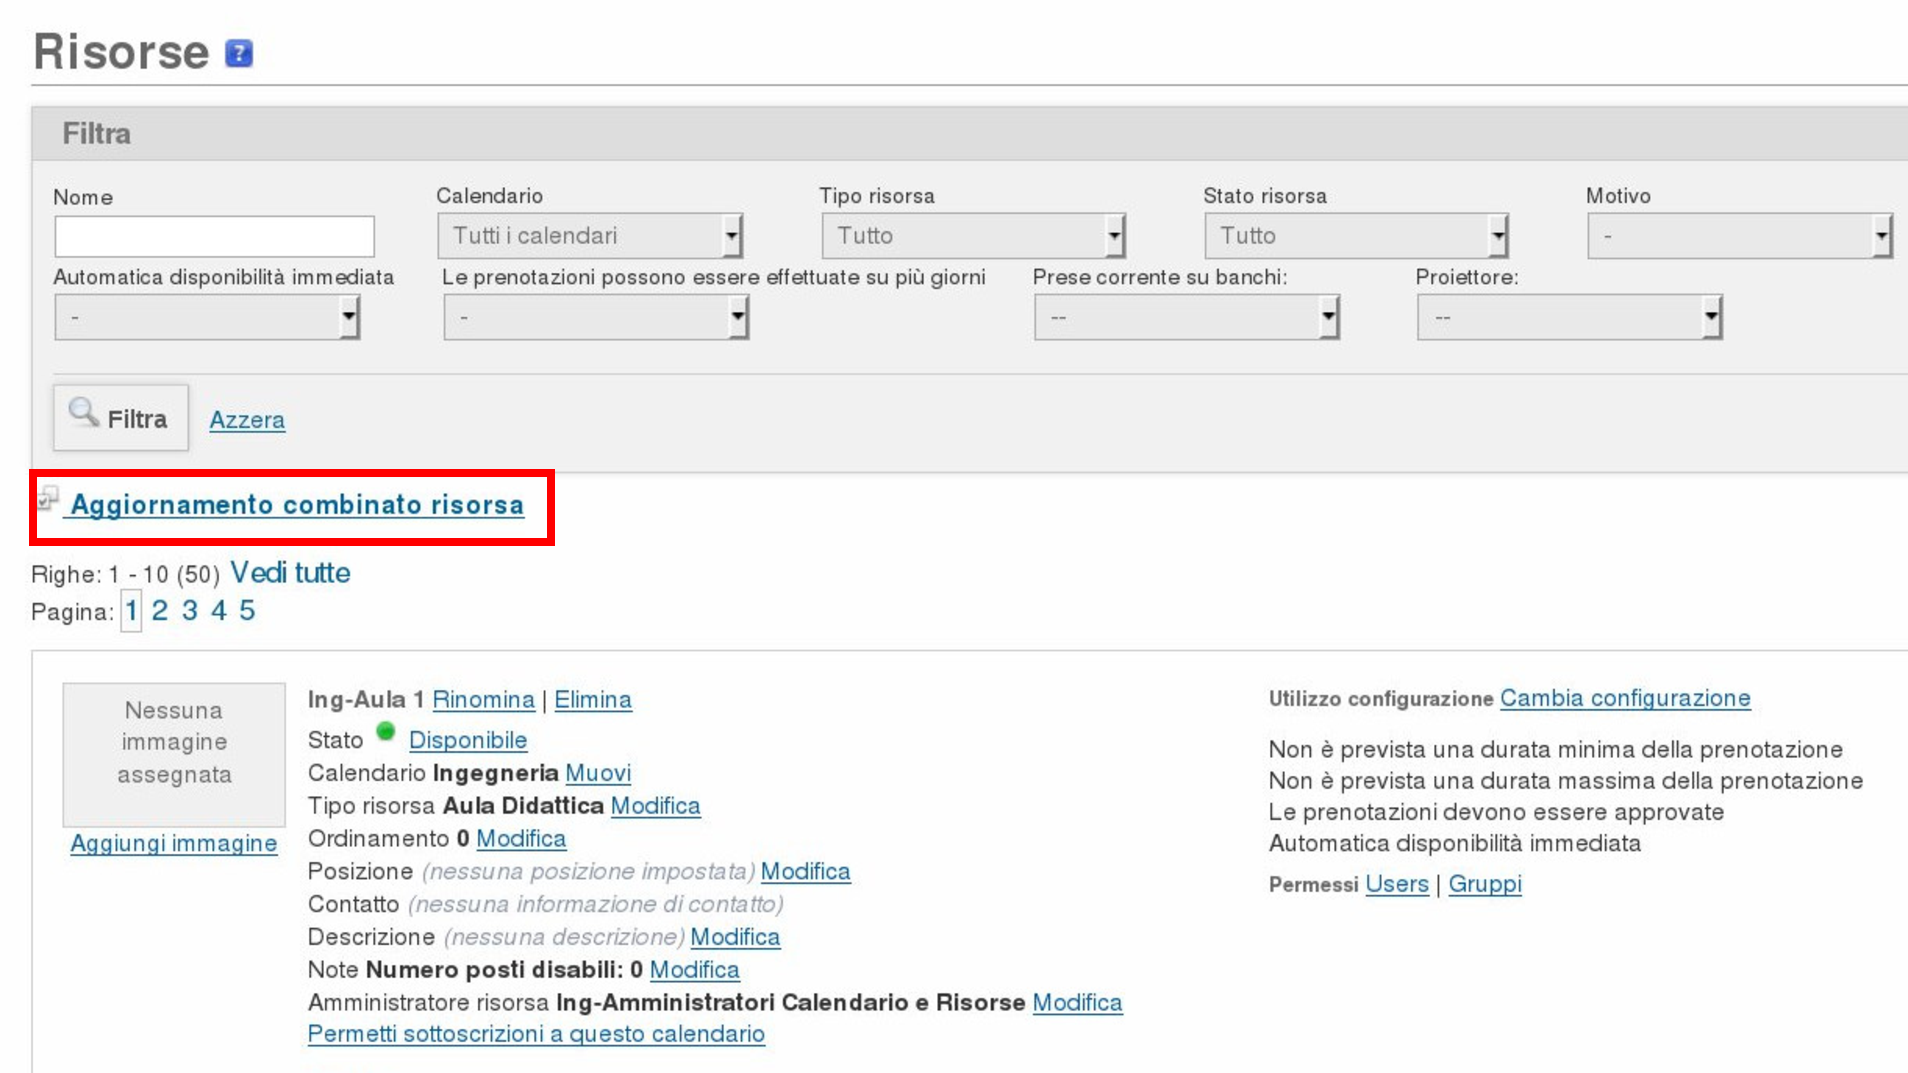
\includegraphics[scale=0.5]{Immagini/risorsa_selezione_configurazione_multipla.pdf}
\normalsize
\caption{}
\label{fig:risorsa_selezione_configurazione_multipla.pdf}
\end{figure}
\section{Gestione credenziali utenti}
Per un'agevole e rapida gestione degli utenti, essi vengono raggruppati
in gruppi. Ai gruppi possono essere attribuite particolari
proprietà (in Booked vengono chiamati ruoli) che poi verranno
riflesse agli utenti in essi contenuti, permettendogli di ampliare l'insieme
delle azioni che possono essere eseguite: I RUOLI POSSONO ESSERE MODIFICATI SOLO
DALL'APPLICATION ADMIN

\begin{figure}[H]
\centering{}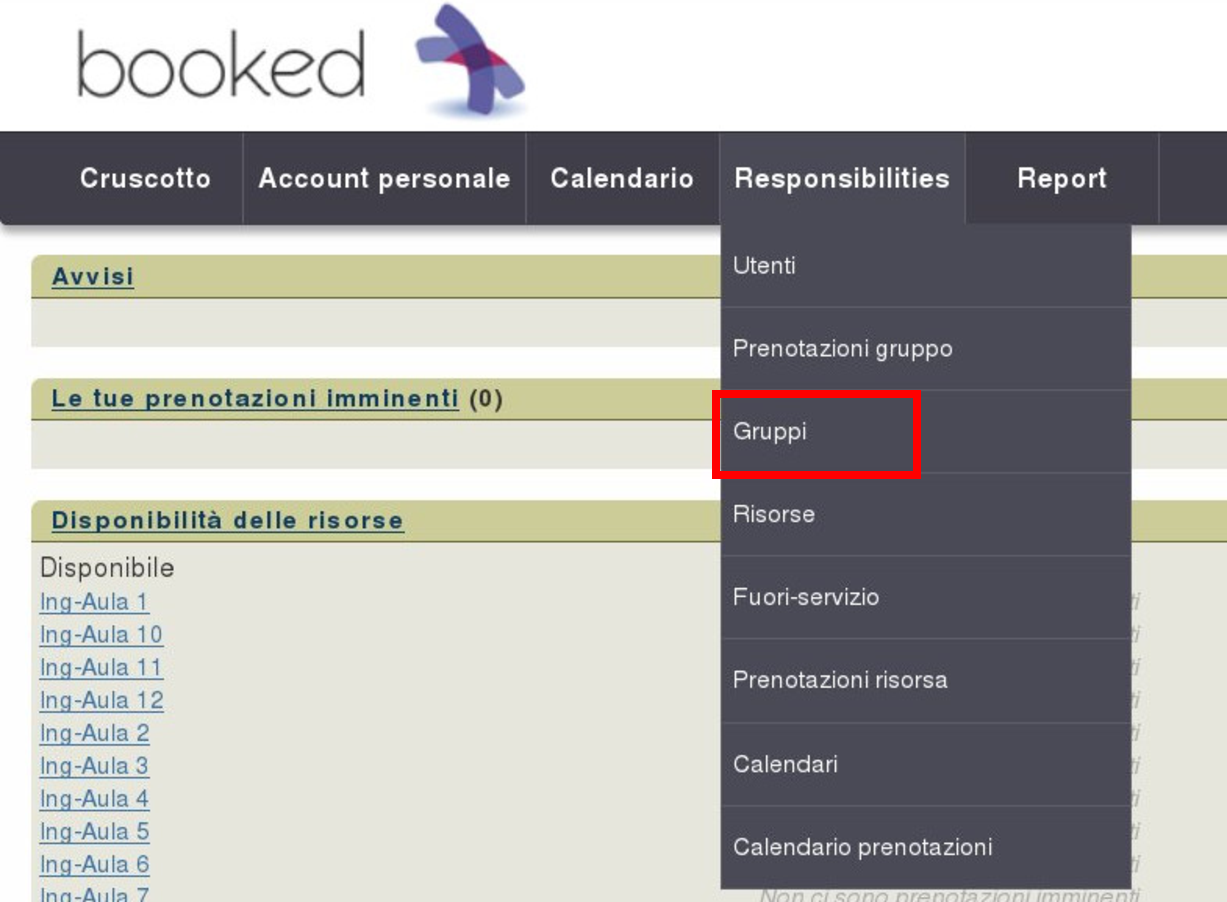
\includegraphics[scale=0.5]{Immagini/amministratore_menu_generale_selezione_gruppi.pdf}
\normalsize
\caption{}
\label{fig:amministratore_menu_generale_selezione_gruppi.pdf}
\end{figure}



\begin{figure}[H]
\centering{}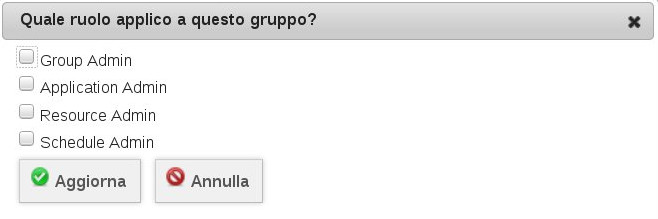
\includegraphics[scale=0.7]{Immagini/ruoli_gruppo.jpeg}
\normalsize
\caption{}
\label{fig:Ruoli assegnabili ad un gruppo}
\end{figure}

\begin{itemize}
 \item Calendar Admin (Amministratore calendario): ogni calendario ha un campo
 ``Amministratore Calendario'' dove si può scegliere uno ed un solo gruppo di utenti
 che ha la proprietà Calendar Admin attiva. Essi possono modificare le proprietà
 del calendario A, come ad esempio le fasce orarie disponibili;
 
 \item Resource Admin (Amministratore risorsa): ogni risorsa ha un campo
 ``Amministratore Risorsa'' dove si può scegliere uno ed un solo gruppo di utenti
 che ha la proprietà Resource Admin attiva. Essi potranno modificare le proprietà
 delle risorse e delle relative prentazioni,
 nonché crearne di nuove;
 
 \item Group Admin (Amministratore gruppo): ogni gruppo di utenti ha un campo
 ``Amministratore Gruppo'' dove si può scegliere uno ed un solo gruppo di utenti
 che ha la proprietà Group Admin attiva. Essi potranno modificare le proprietà
 del gruppo, come ad esempio aggiungere utenti.
 
\end{itemize}
Le proprietà (ruoli) appena elencate non sono strutturate gerarchicamente,
ma li si può abilitare uno alla volta per far sì che un utente possa effettuare
più tipi di azioni.
\paragraph*{Esempio}\mbox{}\\ %per andare a capo dopo nome paragrafo.
Il gruppo utenti con nome ``Amministratori Ingegneria'' possiede attributi Resource Admin e Calendar Admin.
L'utente Carlo fa parte di tale gruppo.
Si ha inoltre:
\begin{itemize}
 \item un calendario ``Ingegneria'' nel cui campo ``Amministratore Calendario''
 è stato impostato che il gruppo di amministratori è ``Amministratori Ingegneria'';
 \item una serie di risorse: Ing-Aula 1, Ing-Aula 2... nel cui campo
 ``Amministratore Risorsa'' è stato impostato che il gruppo di amministratori
 è ``Amministratori Ingegneria'';
\end{itemize}
perciò Carlo potrà sia modificare le risorse che i calendari di Ingegneria in quanto
il suo gruppo di appartenenza possiede le proprietà (ruoli) Resource Admin e Calendar Admin.

\paragraph*{Notare bene:}\mbox{}\\ %per andare a capo dopo nome paragrafo.
\begin{itemize}
 \item qualora il gruppo ``Amministratori Ingegneria'' non avesse avuto tra gli attributi Calendar Admin, non avrebbe potuto
essere selezionato come amministratore del calendario di Ingegneria (né ovviamente di altri);
\item qualora il gruppo ``Amministratori Ingegneria'' non avesse avuto tra gli attributi Resource Admin, non avrebbe potuto
essere selezionato come amministratore delle risorse di Ingegneria (né ovviamente di altre);
\end{itemize}
\end{document}
